%
% problem-discussion.tex
%
% Copyright (C) 2022 by Universidade Federal de Santa Catarina.
%
% GNSS Networks Based on Small Satellites
%
% This work is licensed under the Creative Commons Attribution-ShareAlike 4.0
% International License. To view a copy of this license,
% visit http://creativecommons.org/licenses/by-sa/4.0/.
%

%
% \brief Problem discussion chapter.
%
% \author Gabriel Mariano Marcelino <gabriel.mm8@gmail.com>
%
% \version 0.1.0
%
% \date 2021/06/14
%


\chapter{Problem Discussion} \label{ch:problem-discussion}

%Os sistemas de navegação global por satélite atualmente são largamente utilizados por diversos dispositivos, incluindo desde sistemas complexos como aeronaves, satélites e foguetes, até disponíveis mais simples de uso geral como celulares, computadores, rastreadores de veículos, etc.

%Atualmente existem seis diferentes redes em operação, sendo um tipo de tecnologia dominada por poucos países do mundo. Todas as redes atuais operam com a utilização de satélites de grande porte e operando em órbitas baixas e médias (LEO e MEO).

%Com o surgimento e ascenção dos pequenos satélites, em especial os CubeSats, na última década, surge também a possibilidade de utilizar satélites de menor porte, mais simples e de menor custo para aplicações que anteriormente só poderiam ser solucionadas com satélites de grande porte e custo elevado.

%Especificamente sobre as redes de GNSS, o uso de satélites de pequeno porte pode agregar inúmeras vantagens, sendo umas das principais a redução de custo (tanto de desenvolvimento e operação), e também fácil reposição dos satélites da constelação.

%Este capítulo apresenta uma discussão sobre os principais aspectos e problemas a serem considerados para redes de GNSS no geral, e também mais especificamente uma possível rede baseada em satélites de pequeno porte e/ou operando em órbitas baixas.

Global navigation satellite systems are currently widely used by various devices, including complex systems such as aircraft, satellites, and rockets, as well as simpler devices for general use such as cell phones, computers, vehicle trackers, etc.

Currently, there are six different networks in operation, with the technology dominated by few countries in the world. All current networks operate using large satellites in low and medium orbits (LEO and MEO).

With the emergence and rise of small satellites, especially CubeSats, in the last decade, the possibility of using smaller, simpler, and lower-cost satellites for applications that previously could only be solved with large and costly satellites also arises.

Specifically regarding GNSS networks, the use of small satellites can bring numerous advantages, including the reduction of costs (both development and operation) and easy replacement of constellation satellites.

This chapter presents a discussion of the main aspects and problems to be considered for GNSS networks in general, and also specifically a possible network based on small satellites and/or operating in low orbits.

% #############################################################################
% #############################################################################
% #############################################################################
% #############################################################################

\section{Timing precision}

% https://gssc.esa.int/navipedia/index.php/Precise_Time_Reference#cite_note-About-2

GNSS technologies have a design dependence on accurate timing. The resolution of positioning equations depend on the accurate time stamping of GNSS messages and the four variables resolved by positioning equations are: time plus the 3D position coordinates. Each navigation satellite has atomic clocks that are synchronized from a master clock on the ground and the navigation messages are timestamped with the transmission time of the signal.

This allows GNSS receivers to act as a worldwide synchronized time source with a precision that could only be maintained during long periods by expensive equipments. This enabled a wide set of applications that rely on GNSS synchronized precise time sources. These applications can range from network synchronization and optimization to encryption and digital signature of electronic data.

The receiver's clocks, however, are small quartz oscillators like those found in a wristwatch. Quartz oscillators are very accurate when measuring times of less than a few seconds, but rather inaccurate over longer periods. The solution is to re-set the receiver’s time to the satellite's time continuously. This is done by the receiver's processor using an approximation method involving signals from at least four satellites \cite{gmv2011}.

The accuracy achieved by GNSS-based time synchronization using GPS is lesser than 40 ns at 95 \% of time \cite{gps-standard}.

%A estabilidade do relógio interno de um satélite emissor de sinais de GNSS é atualmente é da ordem de uma a duas partes em $10^{13}$ por dia, ou seja, aproximadamente 8,64 à 17,28 ns por dia. Este valor resulta em erros de localização na ordem de 2,59 à 5,18 m \cite{ahmed2002}. Deste modo, quanto mais preciso for a referência de tempo interna de um satélite que emite sinais de GNSS, maior será a precisão da localização aferida. Outro aspecto importante relacionado, é a correção periódica aplicada ao horário interno do satélite. Estações em terra com referências tempo altamente precisas, precisam periodicamente corrigir o tempo do relógio dos satélites de uma rede GNSS. Quanto maior período das correções, menor será o erro de tempo e consequentemente de localização propagado.

The stability of the internal clock of a GNSS signal-emitting satellite is currently on the order of one to two parts in $10^{13}$ per day, which is approximately 8.64 to 17.28 ns per day. This value results in location errors on the order of 2.59 to 5.18 m \cite{ahmed2002}. Therefore, the more precise the internal time reference of a GNSS signal-emitting satellite, the greater the accuracy of the measured location. Another important aspect is the periodic correction applied to the internal time of the satellite. Ground stations with highly precise time references need to periodically correct the time of the clocks of GNSS network satellites. The longer the correction period, the lower the time error and consequently the propagated location error.

%Outro aspecto que afeta o relógio interno de um satélite é a teoria da relatividade (geral e especial). Em um relógio abordo de um satélite orbitando a Terra pode ser observado uma passagem de tempo de aproximadamente 38,4 $\mu$s/dia mais rápida do que um relógio presente na superfície terrestre. Para compensar esse problema, um leve deslocamento temporal é adicionado ao relógio interno do satélite antes do seu lançamento. Mas um efeito residual ainda ocorre devido a não idealidade da órbita do mesmo, ou seja, objetos orbitando a Terra não seguem uma órbita perfeitamente circular. Desta forma, uma correção pode ser aplicada utilizando a \autoref{eq:orbit-correction} \cite{hauschild2017}.

Another aspect that affects the internal clock of a satellite is the theory of relativity (general and special). On a clock aboard a satellite orbiting the Earth, a passage of time approximately 38.4 $\mu$s/day faster than a clock on the Earth's surface can be observed. To compensate for this problem, a slight time shift is added to the satellite's internal clock before its launch. However, a residual effect still occurs due to the non-ideality of its orbit, i.e., objects orbiting the Earth do not follow a perfectly circular orbit. Thus, a correction can be applied using \autoref{eq:orbit-correction} \cite{hauschild2017}.

\begin{equation} \label{eq:orbit-correction}
    \Delta t_{r} = - \frac{2}{c^{2}} \sqrt{\mu a} (e \sin{E})
\end{equation}

Where:

\begin{itemize}
    \item $c$ is the speed of light
    \item $\mu$ is the universal gravitational constant of Earth ($3.986005 \times 10^{14}\ m^{3}/s^{2}$)
    \item $a$ is the semi-major axis of Earth
    \item $e$ is the eccentricity of the satellite's orbit
    \item $E$ is the eccentric anomaly of the satellite's orbit
\end{itemize}

%Também é possível utilizar a própria velocidade e posição do satélite para se obter a correção relativística, usando a \autoref{eq:orbit-correction-alt} \cite{icd2010navstar}.

It is also possible to use the satellite's own velocity and position to obtain the relativistic correction, using \autoref{eq:orbit-correction-alt} \cite{icd2010navstar}.

\begin{equation} \label{eq:orbit-correction-alt}
    \Delta t_{r} = -\frac{2 r^{s} \cdot v^{s}}{c^{2}}
\end{equation}

%Onde $r^{s} \cdot v^{s}$ é o produto escalar dos vetores de posição ($r^{s}$) e velocidade ($v^{s}$) do satélite.

Where $r^{s} \cdot v^{s}$ is the dot product of the position vector ($r^{s}$) and velocity vector ($v^{s}$) of the satellite, and $c$ is the speed of light.

% #############################################################################
% #############################################################################
% #############################################################################
% #############################################################################

\section{Ionospheric delay} \label{sec:ionospheric-delay}

%Um outro aspecto que afeta o desempenho e o funcionamento dos sistemas de GNSS é o atraso causado pela ionosfera, que ocorre pela refração causada quando os sinais transmitidos pelos satélites de um sistema de navegação atravessam essa camada da atmosfera, localizada entre 50 e 1000 km de altitude em relação a superfície terrestre. Como indicado pelo nome, a ionosfera é um meio parcialmente ionizado, resultado dos raios X e UV da radiação solar e da incidência de partículas carregadas.

%A velocidade de propagação de um sinal que passa pela ionosfera depende basicamente da densidade de elétrons da mesma, que varia de acordo com os ciclos diurnos e noturnos. Quando uma região está sob o dia, a incidência de radiação solar causa a ionização de átomos eletricamente neutros, o que provoca elétrons livres e íons. E quando a mesma região passa a estar no período noturno ocorre o processo inverso: elétrons livre se recombinam com íons para formar partículas neutras novamente. Este processo tem como resultado a variação da densidade de elétrons ao longo dessa camada.

%Essa também é considerada uma das principais fontes de erro nos sistema de localização por satélite. Devido a natureza da refração, este tipo problema afeta em maior grau sinais vindo do horizonte, ou seja, quando um satélite passa com uma elevação mais baixa. Já sinais vindo de altas elevações são afetados em menor grau por esse tipo de problema. Ou seja, quanto maior for o tempo em que um sinal está dentro da ionosfera, maiores são os efeitos causados pela mesma. Como resultado, o caminho percorrido por um sinal passa a ser maior, e consequentemente o tempo total de deslocamento também aumenta, alterando a estimativa de distância entre o satélite emissor do sinal e um receptor em terra. Este atraso também pode variar principalmente de acordo com a hora do dia, a época do ano, a região e a atividade solar.

%A refração dos sinais de GNSS também depende da frequência em que os sinais são transmitidos. Frequências maiores são menos afetadas que frequências menores. Essa relação pode ser descrita através da \autoref{eq:ionospheric-delay-freq} \cite{brunner1993}.

Another aspect that affects the performance and operation of GNSS systems is the delay caused by the ionosphere, which occurs due to refraction when signals transmitted by navigation system satellites cross this layer of the atmosphere, located between 50 and 1000 km in altitude relative to the earth's surface. As indicated by the name, the ionosphere is a partially ionized medium, resulting from X-rays and UV\nomenclature{\textbf{UV}}{Ultra Violet.} radiation from the sun and the incidence of charged particles.

The propagation speed of a signal that passes through the ionosphere depends mainly on its electron density, which varies according to daily and nocturnal cycles. When a region is under daylight, the incidence of solar radiation causes the ionization of electrically neutral atoms, which leads to free electrons and ions. And when the same region becomes nocturnal, the opposite process occurs: free electrons recombine with ions to form neutral particles again. This process results in a variation in electron density along this layer.

This is also considered one of the main sources of error in satellite-based location systems. Due to the nature of refraction, this type of problem affects signals coming from the horizon to a greater extent, i.e., when a satellite passes with lower elevation. Signals from high elevations are affected to a lesser extent by this type of problem. Therefore, the longer a signal is within the ionosphere, the greater the effects caused by it. As a result, the path traveled by a signal becomes longer, and consequently, the total travel time also increases, altering the distance estimate between the satellite emitting the signal and a receiver on the ground. This delay can also vary mainly according to the time of day, the time of year, the region, and solar activity.

The refraction of GNSS signals also depends on the frequency at which the signals are transmitted. Higher frequencies are less affected than lower frequencies. This relationship can be described by equation \ref{eq:ionospheric-delay-freq} \cite{brunner1993}.

\begin{equation} \label{eq:ionospheric-delay-freq}
    v = \frac{40.3}{cf^{2}} \cdot TEC
\end{equation}

Where:

\begin{itemize}
    \item $v$ is the delay caused by the ionosphere
    \item $c$ is the speed of light in meters per second
    \item $f$ is the frequency of the signal in Hertz
    \item $TEC$ is the total electron content per square meter
\end{itemize}

%Utilizando duas frequências distintas, esta dependência pode ser reduzida em até 99,9 \% \cite{ionospheric-delay-navipedia}. Neste caso, há a necessidade também da utilização de receptores que operam duas frequências. Também é possível a implementação de sistemas que operam somente em uma frequência, onde neste caso é necessária a utilização de modelos de ionosfera para prever e reduzir a incidência deste efeito.

%Como a ionosfera também engloba satélites de órbita de baixa, este é um problema que afeta de forma semelhante satélites de grande porte operando em órbitas MEO, e satélite de pequeno porte operando tanto em MEO quanto em LEO. Mas considerando que a ionosfera também pode ser dividida em subcamadas, sinais sendo emitidos em órbitas mais baixas e de ``dentro'' da própria ionosfera tendem a ter uma menor influência dos atrasados causados pela mesma, já que o tempo de permanência do sinal dentro da camada acaba sendo menor. Mais especificamente, considera-se a subdivisão em três subcamadas \cite{geog862}: região D, E e F, sendo a primeira na faixa aproximada de 50 à 90 km, a segunda entre 90 e 120 km, e a terceira entre 120 e 1000 km. A primeira camada praticamente não afeta os sinais de GNSS, a segunda tem um efeito pequeno sobre os sinais, e a terceira é a camada predomina e que causa os maiores atrasos por conter a maior concentração de ionização. Esta última camada também pode ser dividida em regiões menores (F1 e F2), que possuem densidades diferentes de acordo com a época do ano ou horário do dia.

Using two distinct frequencies, this dependence can be reduced by up to 99.9 \% \cite{ionospheric-delay-navipedia}. In this case, the use of receivers that operate at two frequencies is also necessary. It is also possible to implement systems that operate at only one frequency, in which case ionosphere models are needed to predict and reduce the incidence of this effect \cite{rao2008}.

Since the ionosphere also includes low-orbit satellites, this is a problem that affects both large satellites operating in MEO orbits and small satellites operating in both MEO and LEO. However, considering that the ionosphere can also be divided into sub-layers, signals being emitted in lower orbits and ``inside'' the ionosphere itself tend to have less influence from delays caused by it, since the time the signal stays inside the layer is shorter. Specifically, it is divided into three sub-layers \cite{geog862}: region D, E, and F, with the first in the approximate range of 50 to 90 km, the second between 90 and 120 km, and the third between 120 and 1000 km. The first layer practically does not affect GNSS signals, the second has a small effect on the signals, and the third is the predominant layer that causes the greatest delays due to containing the highest ionization concentration. This last layer can also be divided into smaller regions (F1 and F2), which have different densities according to the time of year or time of day.

\begin{figure}[!ht]
    \begin{center}
        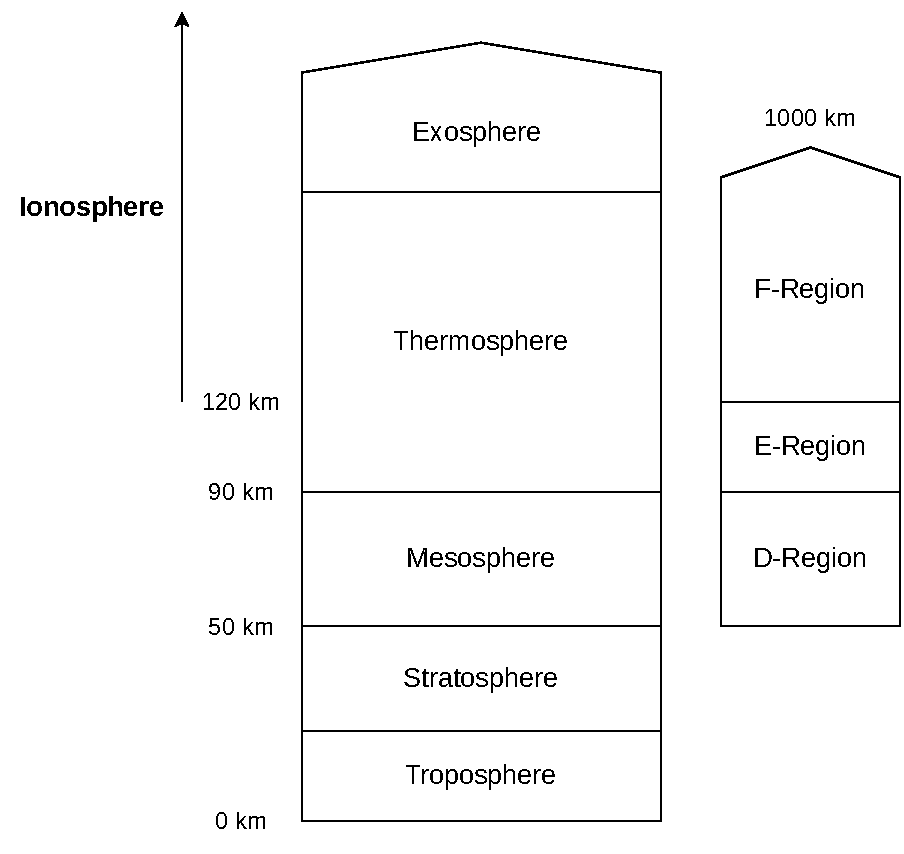
\includegraphics[width=0.6\columnwidth]{figures/atmosphere-model.pdf}
        \caption{Atmosphere model (adapterd from \cite{geog862}).}
        \label{fig:atmosphere-model}
    \end{center}
\end{figure}

% #############################################################################
% #############################################################################
% #############################################################################
% #############################################################################

\section{Telecommunication analysis} \label{sec:telecom-analysis-method}

%Outro aspecto de vital importância para o funcionamento de redes de GNSS está relacionado ao enlace de comunicação entre o satélite e um receptor em terra. Considerando que um satélite de uma rede deste tipo operar em uma altitude de centenas de quilômetros ou até mesmo na faixa dos milhares de quilômetros, a potência do sinal recebido por um receptor em solo é baixa. Para o correto funcionamento do enlace, a potência transmitida, a modulação e os possíveis protocolos envolvidos devem ser compatíveis. Nesta seção apresenta-se os cálculos relacionados ao link budget. O procedimento aqui adotado é o mesmo apresentado em \cite{larson2005}.

Another aspect of vital importance for the functioning of GNSS networks is related to the communication link between the satellite and a ground receiver. Considering that a satellite in such a network operates at an altitude of hundreds or even thousands of kilometers, the power of the signal received by a ground receiver is low. For the link to work correctly, the transmitted power, modulation, and possible protocols involved must be compatible. This section presents the calculations related to the link budget. The procedure adopted here is the same as presented in \cite{larson2005}.

\subsection{Distance to satellite at horizon}

First, the distance between the satellite and a potential receiver must be determined. This distance varies according to the altitude of the satellite and its elevation along the orbit. This way, the distance to satellite at horizon (the maximum theoretical distance between the satellite and a receiver on Earth) can be calculated using \autoref{eq:horizon-distance}.

\begin{equation} \label{eq:horizon-distance}
d = \sqrt{2\cdot R_{e}\cdot h + h^{2}}
\end{equation}

Where:

\begin{itemize}
    \item $R_{e}$ = Earth radius $\cong$ 6378 km
    \item $h$ = Satellite altitude
    \item $d$ = Distance to sattellite at horizon
\end{itemize}

\subsection{Free-Space Path Loss}

The free-space path loss ($FSPL$\nomenclature{\textbf{FSPL}}{Free-Space Path Loss.}) can be calculated using \autoref{eq:fspl}.

\begin{equation} \label{eq:fspl}
FSPL = \left( \frac{4\pi d f}{c} \right)^{2}
\end{equation}

Where:

\begin{itemize}
    \item $d$ = Distance between the satellite and the receiver
    \item $f$ = Radio frequency
    \item $c$ = Speed of light
\end{itemize}

The FSPL value in decibels can be calculated with \autoref{eq:fsbl-db}.

\begin{equation} \label{eq:fsbl-db}
    \begin{split}
        FSPL^{dB} & = 20 \cdot \log\left(\frac{4\pi}{c}\right) + 20 \cdot \log\left(d\right) + 20 \cdot \log\left(f\right) \\
                  & = 32,45 + 20 \cdot \log\left(\frac{d^{km}}{1\ km}\right) + 20 \cdot \log\left(\frac{f^{MHz}}{1\ MHz}\right) \\
    \end{split}
\end{equation}

The minimum distance between the satellite and a receiver is the satellite altitude. The maximum distance is the distance at horizon, defined by \autoref{eq:horizon-distance}.

\subsection{Power at receiver}

The power of the signal at the receiver can be estimated using \autoref{eq:power-at-receiver}.

\begin{equation} \label{eq:power-at-receiver}
    P_{r} = P_{t} + G_{t} + G_{r} - L_{p} - L_{s}
\end{equation}

Where:

\begin{itemize}
    \item $P_{r}$ = Power at the receiver
    \item $P_{t}$ = Transmitter power
    \item $G_{t}$ = Antenna gain of the transmitter
    \item $G_{r}$ = Antenna gain of the receiver
    \item $L_{p}$ = FSPL (Free-Space Path Loss)
    \item $L_{s}$ = Other losses in the system
\end{itemize}

\subsection{Signal-to-Noise-Ratio}

The Signal-to-Noise-Ratio (SNR\nomenclature{\textbf{SNR}}{Signal-to-Noise-Ratio.}) of a transmitted signal at the receiver can be expressed using \autoref{eq:snr}.

\begin{equation} \label{eq:snr}
    SNR = \frac{E_{b}}{N_{0}} = \frac{P_{t}G_{t}G_{r}}{kT_{s}RL_{p}}
\end{equation}

Where:

\begin{itemize}
    \item $P_{t}$ = Transmitter power
    \item $G_{t}$ = Antenna gain of the transmitter
    \item $G_{r}$ = Receiver gain
    \item $k$ = Boltzmann's constant ($\cong 1,3806 \times 10^{-23}\ J/K$)
    \item $T_{s}$ = System noise temperature
    \item $R$ = Data rate in bits per seconds (bps)
    \item $L_{p}$ = Free-Space Path Loss (FSPL)
\end{itemize}

The system noise temperature ($T_{s}$) can be defined using \autoref{eq:system-noise-temperature}.

\begin{equation} \label{eq:system-noise-temperature}
    T_{s} = T_{ant} + T_{r}
\end{equation}

with:

\begin{equation} \label{eq:noise-temperature-receiver}
    T_{r} = \frac{T_{0}}{L_{r}} (F - L_{r})
\end{equation}

and:

\begin{equation} \label{eq:noise-figure}
    F = 1 + \frac{T_{r}}{T_{0}}
\end{equation}

Combining Equations \ref{eq:system-noise-temperature}, \ref{eq:noise-temperature-receiver} and \ref{eq:noise-figure}:

\begin{equation} \label{eq:system-noise-temp-expanded}
    T_{s} = T_{ant} + \left( \frac{T_{0}(1 - L_{r})}{L_{r}} \right) + \left( \frac{T_{0} (F - 1)}{L_{r}} \right)
\end{equation}

Where:

\begin{itemize}
    \item $T_{ant}$ = Antenna noise temperature
    \item $T_{0}$ = Reference temperature (usually 290 K)
    \item $L_{r}$ = Line loss between the antenna and the receiver
    \item $F$ = Noise figure of the receiver
    \item $T_{r}$ = Noise temperature of the receiver
\end{itemize}

The SNR value in decibels can be calculated using the \autoref{eq:snr-db}:

\begin{equation} \label{eq:snr-db}
    \begin{split}
        SNR^{dB} & = 10 \cdot \log_{10}\left( \frac{E_{b}}{N_{0}} \right) = 10 \cdot \log_{10} \left( \frac{P_{t}G_{t}G_{r}}{kT_{s}RL_{p}} \right) \\
                 & = P_{t}^{dBm} - 30 + G_{t}^{dB} + G_{r}^{dB} - L_{p}^{dB} - 10 \cdot \log k - 10 \cdot \log T_{s} - 10 \cdot \log R
    \end{split}
\end{equation}

Considering other losses in the system ($L_{s}$) (cable and connection losses as example), the \autoref{eq:snr-db} can be corrected as presented in \autoref{eq:snr-db-with-losses}.

\begin{equation} \label{eq:snr-db-with-losses}
    SNR^{dB} = P_{t}^{dBm} - 30 + G_{t}^{dB} + G_{r}^{dB} - L_{p}^{dB} - L_{s}^{dB} - 10 \cdot \log k - 10 \cdot \log T_{s} - 10 \cdot \log R
\end{equation}

\subsection{Link margin}

From \cite{larson2005}, the minimum SNR value at the received considering a $10^{-5}$ bit error rate for several type of modulation and coding schemes is available in \autoref{tab:link-margins}.

\begin{table}[!ht]
    \centering
    \begin{tabular}{lC{0.2\textwidth}C{0.2\textwidth}}
        \toprule[1.5pt]
        \textbf{Modulation} & \textbf{$\mathbf{E_{b}/N_{0}}$ for BER = $\mathbf{10^{-5}}$ [dB]} & \textbf{Spectrum utilization} \\
        \midrule
        BPSK                            & 9.6  & 1.0 \\
        DPSK                            & 10.3 & 1.0 \\
        QPSK                            & 9.6  & 2.0 \\
        FSK                             & 13.3 & 0.5 \\
        8FSK                            & 9.2  & 0.375 \\
        BPSK and QPSK $+$ R-1/2 Viterbi & 4.4  & 0.5 and 1.0 \\
        BPSK $+$ RS Viterbi             & 2.7  & 0.44 \\
        MSK                             & 9.6  & 1.5 \\
        \bottomrule[1.5pt]
    \end{tabular}
    \caption{Minimum link margins for several modulation and coding schemes (adapted from \cite{larson2005}).}
    \label{tab:link-margins}
\end{table}

So, the link margin can be obtained by the difference between the SNR and the respective $E_{b}/N_{0}$ value for the communication scheme.

% #############################################################################
% #############################################################################
% #############################################################################
% #############################################################################

\section{Power consumption analysis}

%Um dos aspectos de vital importância nos satélites em geral é a relação entre o consumo e a geração de energia. Especialmente em pequenos satélites, esse aspecto se torna ainda mais relevante e requer ainda mais atenção, devido principalmente ao tamanho reduzido e consequentemente menor capacidade de geração de energia (um volume menor leva a uma menor área disponível para painéis solares).

%Desta forma, uma das principais análises a ser feita para o projeto de uma missão espacial é o power budget, com o objetivo de garantir uma margem positiva de energia ao longo de toda vida útil do satélite.

One of the crucial aspects in satellites in general is the relationship between power consumption and energy generation. Especially in small satellites, this aspect becomes even more relevant and requires even more attention, mainly due to the reduced size and consequently lower energy generation capacity (a smaller volume leads to a smaller area available for solar panels).

Thus, one of the main analyses to be performed for the design of a space mission is the power budget, with the aim of ensuring a positive energy margin throughout the entire useful life of the satellite.

According to section 10.3 of \cite{larson2005}, the power budget of satellite can be determined through three steps:

\begin{enumerate}
    \item Prepare operating power budget
    \item Size the battery
    \item Estimate power degradation over mission life
\end{enumerate}

\subsection{Input power}

%A potência de entrada é o quanto o satélite gera de energia através de seus painéis solares em média ao longo de uma órbita. Dependendo do tipo de órbita, quando o satélite está do lado da Terra em que o Sol está incidindo, há captação de energia solar e armazenamento da mesma nas baterias internas. Nesta fase, o balanço de energia deve ser positivo. Já durante o período em que o satélite está no lado escuro da Terra, praticamente não há captação de energia solar e o balanço de energia torna-se negativo. Levando em conta as duas fases, para o correto funcionamento e durabilidade da missão, o balanço de energia geral ao longo de uma órbita de ser positivo.

%Para se estimar o quanto de energia o satélite irá captar, vários aspectos devem ser levados em conta, como:

%\begin{itemize}
%    \item Tipo de painel solar utilizado (eficiência do mesmo)
%    \item Área dos painéis solares (total e em cada face)
%    \item Geometria do satélite e consequentemente dos painéis solares instalados
%    \item Atitude do satélite ao longo das órbitas
%\end{itemize}

%Para este trabalho, será utilizado o método apresentado em \cite{rigo2023} para se estimar a potência média gerado pelo satélite ao longo de uma órbita para uma determinada configuração e operação do mesmo.

%Por exemplo, para as condições abaixo, tem-se como resultado a curva de geração de energia da \autoref{fig:simulation-input-power-example}.

The input power is how much energy the satellite generates through its solar panels on average throughout an orbit. Depending on the type of orbit, when the satellite is on the side of the Earth where the Sun is shining, there is solar energy capture and storage in the internal batteries. At this stage, the energy balance must be positive. During the period when the satellite is on the dark side of the Earth, there is practically no solar energy capture, and the energy balance becomes negative. Taking into account both phases, for the correct operation and durability of the mission, the overall energy balance over an orbit must be positive.

To estimate how much energy the satellite will capture, several aspects must be taken into account, such as:

\begin{itemize}
    \item Type of solar panel used (its efficiency)
    \item Area of the solar panels (total and on each face)
    \item Geometry of the satellite and therefore the installed solar panels
    \item Attitude of the satellite throughout the orbits
\end{itemize}

For this work, the method presented in \cite{rigo2023} will be used to estimate the average power generated by the satellite over an orbit for a given configuration and operation of the satellite.

For example, for the conditions below, the energy generation curve in \autoref{fig:simulation-input-power-example} is obtained.

\begin{itemize}
    \item Solar irradiance: 1367 $W/m^{2}$
    \item Solar cells efficiency: 30 \%
    \item Total solar cell area: 0.01 $m^{2}$
    \item Timestep: 10 sec
    \item Orbit: Polar with 90$^{\circ}$ of inclination and 550 km of altitude
\end{itemize}

\begin{figure}[!ht]
    \begin{center}
        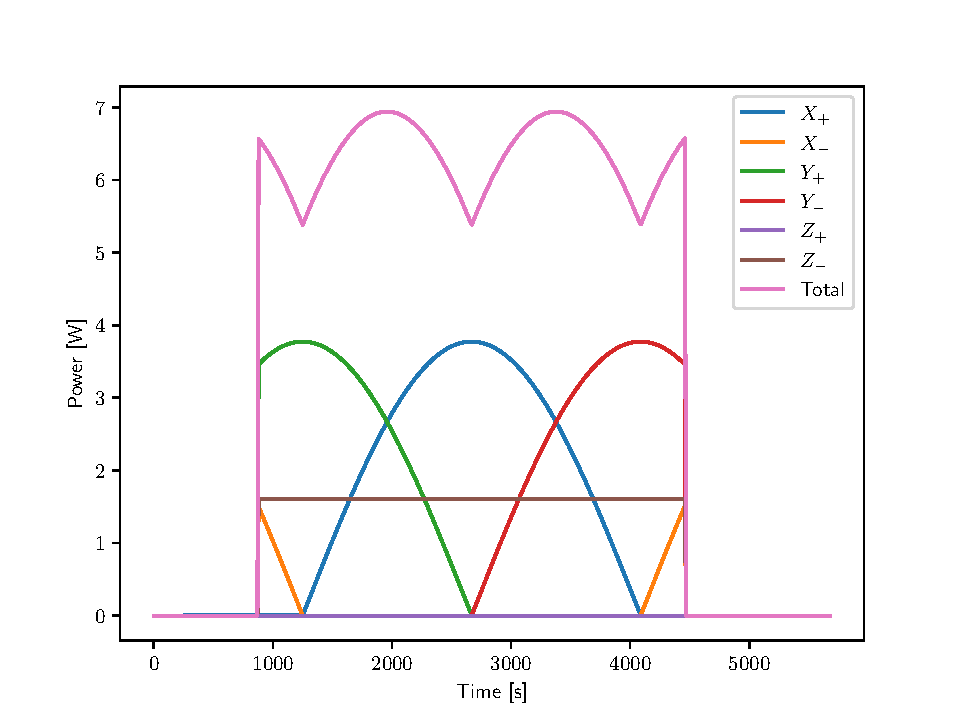
\includegraphics[width=0.9\textwidth]{figures/sim-input-power-3u}
        \caption{Simulated input power of the solar panels using the work of \cite{rigo2023}.}
        \label{fig:simulation-input-power-example}
    \end{center}
\end{figure}

\subsection{Operating power budget}

%Para se obter o orçamento de energia do satélite, precisa-se obter ou estimar os consumos de energia de cada subsistema, juntamente com o quanto cada um ficará ligado durante a operação do mesmo (ou considerar diferentes modos de operação com diferentes consumos para cada subsistema se for o caso).

%Para isso, deve-se ter primeiramente ter os valores de consumo de cada elemento do satélite, e a partir do conceito de operações (CONOPS) definir quanto tempo cada um ficará ligado, na forma de porcentagem em relação ao período de órbita (duty cycle).

To obtain the power budget of the satellite, it is necessary to obtain or estimate the power consumption of each subsystem, along with how long each will be powered on during its operation (or consider different operating modes with different consumption levels for each subsystem if applicable).

To do this, you must first have the power consumption values for each element of the satellite, and based on the concept of operations (CONOPS\nomenclature{\textbf{CONOPS}}{Concept of Operations.}), define how long each will be powered on, in the form of a percentage relative to the orbital period (duty cycle).

Um exemplo pode ser visto na \autoref{tab:power-budget-golds-ufsc}, onde tem-se o power budget previsto para o nanossatélite GOLDS-UFSC \cite{spacelab2022}.

\begin{table}[!ht]
    \centering
    \begin{tabular}{lccccc}
        \toprule[1.5pt]
        \textbf{Module} & \textbf{Duty Cycle [\%]}    & \textbf{Power [mW]} \\
        \midrule
        OBDH                    & 100   & 115 \\
        TTC (radio 1 RX)        & 95    & 65 \\
        TTC (radio 1 TX)        & 5     & 3250 \\
        TTC (radio 2 RX)        & 95    & 65 \\
        TTC (radio 2 TX)        & 5     & 3250 \\
        EPS                     & 100   & 320 \\
        BAT (idle)              & 90    & 0 \\
        BAT (heater full)       & 10    & 5000 \\
        Antenna (deployment)    & 0     & 1800 \\
        Antenna (deployed)      & 100   & 35 \\
        Payload EDC             & 100   & 1250 \\
        Radiation instrument    & 0     & 1000 \\
        \cmidrule{2-3}
        Satellite               & \multicolumn{2}{c}{$\cong$ 2668 mW} \\
        \bottomrule[1.5pt]
    \end{tabular}
    \caption{Power consumption of the subsystems and payloads of the nanosatellite GOLDS-UFSC.}
    \label{tab:power-budget-golds-ufsc}
\end{table}

By utilizing the mean power consumption of the satellite and the mean power generation per orbit, we can achieve power balance within one orbit. If the satellite has more than one mode of operation, this process must be carried out for each mode.

%Para um correto dimensionamento energético, a degradação dos elementos de geração de energia, como os painéis solares, deve ser levada em conta. Dessa forma, para garantir um balanço de energia positivo ao longo de toda vida útil do satélite, deve-se garantir a queda na captação e geração de energia ao final da vida útil. 

For accurate energy sizing, the degradation of energy generation elements, such as solar panels, must be taken into account. Therefore, to ensure a positive energy balance throughout the satellite's entire lifespan, a decrease in energy capture and generation at the end of its life must be guaranteed. From \cite{larson2005}, 5 \% per year is a usual number for the solar panels’ degradation, in other words, the general efficiency of the solar panels decays at a rate of 5 \% per year of operation.

%Com os valores de geração de energia e consumo definidos, o próximo passo é o dimensionamento da bateria do satélite, que armazena energia quando o mesmo está captando energia solar, e fornece energia para toda a eletrônica quando o satélite está em um momento de eclipse. Do mesmo modo, o balanço de energia deve se manter positivo entre as fases de carga e descarga das baterias, ou seja, deve-se garantir que o consumo de energia durante a descarga seja menor que a entrada de energia durante a carga. Dependendo da tecnologia utilizada, também deve-se garantir alguns aspectos de operação, como por exemplo um valor de carga mínimo armazenada na bateria e uma temperatura de operação adequada. E da mesma forma que os painéis solares, também deve se considerar a degradação da mesma ao longo da vida útil do satélite. Normalmente considera-se uma uma taxa de perda de armazenamento de 10 \% ao ano.

With the defined values of energy generation and consumption, the next step is the sizing of the satellite's battery, which stores energy when the satellite is capturing solar energy and supplies power to all electronics during eclipse periods. Similarly, the energy balance must remain positive between the charging and discharging phases of the batteries. This means that the energy consumption during discharge should be lower than the energy input during charging. Depending on the technology used, certain operational aspects must also be ensured, such as a minimum charge value stored in the battery and an appropriate operating temperature. Additionally, like solar panels, the battery's degradation over the satellite's lifespan must also be taken into consideration. Typically, a storage loss rate of 10 \% per year is considered\footnote{The capacity degradation rate of the batteries depends on a lot of variables, like temperature variation, the number of charge and discharge cycles, and so on.}.

% #############################################################################
% #############################################################################
% #############################################################################
% #############################################################################

\section{Orbit analysis}

%Por fim, uma análise também de extrema importância para um correto projeto e dimensionamento de um satélite é a análise de órbita. A órbita em que o satélite irá operar influência por exemplo nos canais de comunicação e na geração de energia. Além disso, está diretamente relacionada com o propósito e o plano de operação do satélite, determinando muitas vezes por quanto tempo o satélite permanecerá em operação.

%Para um satélite com o objetivo de transmitir sinais de geolocalização para qualquer região do planeta, deseja-se que o mesmo tenha uma cobertura a nível global e que consiga transmitir os seus sinais para qualquer região do globo. Desta forma, a órbita escolhida deve levar este ponto em consideração. No caso deste trabalho, umas das possibilidades é a da utilização de órbitas baixas, um tipo de órbita que se adequá nesse requisito são as órbitas polares, com um ângulo de inclinação próximo dos 90$^{\circ}$.

%Para o caso de sistemas regionais, outros tipos de órbitas podem ser levadas em consideração, como por exemplo elevações mais baixas e/ou diferentes valores de apogeu e perigeu, para cobrir só uma faixa ou região específica do globo.

%Para realizar esse tipo de análise, normalmente se recorre a software de simulações de órbita. Há diversas aplicações disponíveis atualmente, mas entre as mais usadas por se destacar o STK \cite{STK} e o FreeFlyer \cite{freeflyer}, que são ferramentas comerciais, e o GMAT \cite{gmat} que é uma ferramenta aberta.

Finally, an analysis of utmost importance for the correct design and sizing of a satellite is the orbit analysis. The orbit in which the satellite will operate influences, for example, the communication channels and power generation. Moreover, it is directly related to the purpose and operational plan of the satellite, often determining how long the satellite will remain in operation.

For a satellite aiming to transmit geolocation signals to any region of the planet, it is desired to have global coverage and be able to transmit its signals to any part of the globe. Therefore, the chosen orbit must take this into consideration. In the case of this work, one possibility is the use of low orbits, specifically polar orbits with an inclination angle close to 90 degrees, as they are suitable for meeting this requirement.

For regional systems, other types of orbits can be considered, such as lower elevations and/or different values of apogee and perigee, to cover only a specific range or region of the globe.

To perform this type of analysis, orbit simulation software is commonly used. There are several applications available today, but among the most widely used are the commercial tools STK\nomenclature{\textbf{STK}}{System Took Kit.} (Systems Tool Kit) \cite{STK} and FreeFlyer \cite{freeflyer}, as well as the open-source tool GMAT\nomenclature{\textbf{GMAT}}{General Mission Analysis Tool.} (General Mission Analysis Tool) \cite{gmat}.